% ================= SEKCJA 8 =================
\section{Model danych i diagram ERD}

Model danych stanowi podstawę działania systemu \texttt{WorkFlow}. To w bazie danych przechowywane są informacje o pracownikach, zakładach, projektach, umowach, certyfikatach, dokumentach, nieobecnościach, zdarzeniach RCP, wpisach czasu pracy oraz eksportach rozliczeniowych. Poprawne zaprojektowanie relacji pomiędzy tymi danymi ma bezpośredni wpływ na spójność systemu oraz możliwość dalszego rozwoju aplikacji.

W projekcie wykorzystano relacyjną bazę danych PostgreSQL oraz narzędzie Prisma ORM. Schemat bazy został zdefiniowany w pliku \texttt{schema.prisma}, natomiast graficzna reprezentacja modelu została przygotowana w postaci diagramu ERD.

\begin{figure}[H]
    \centering
    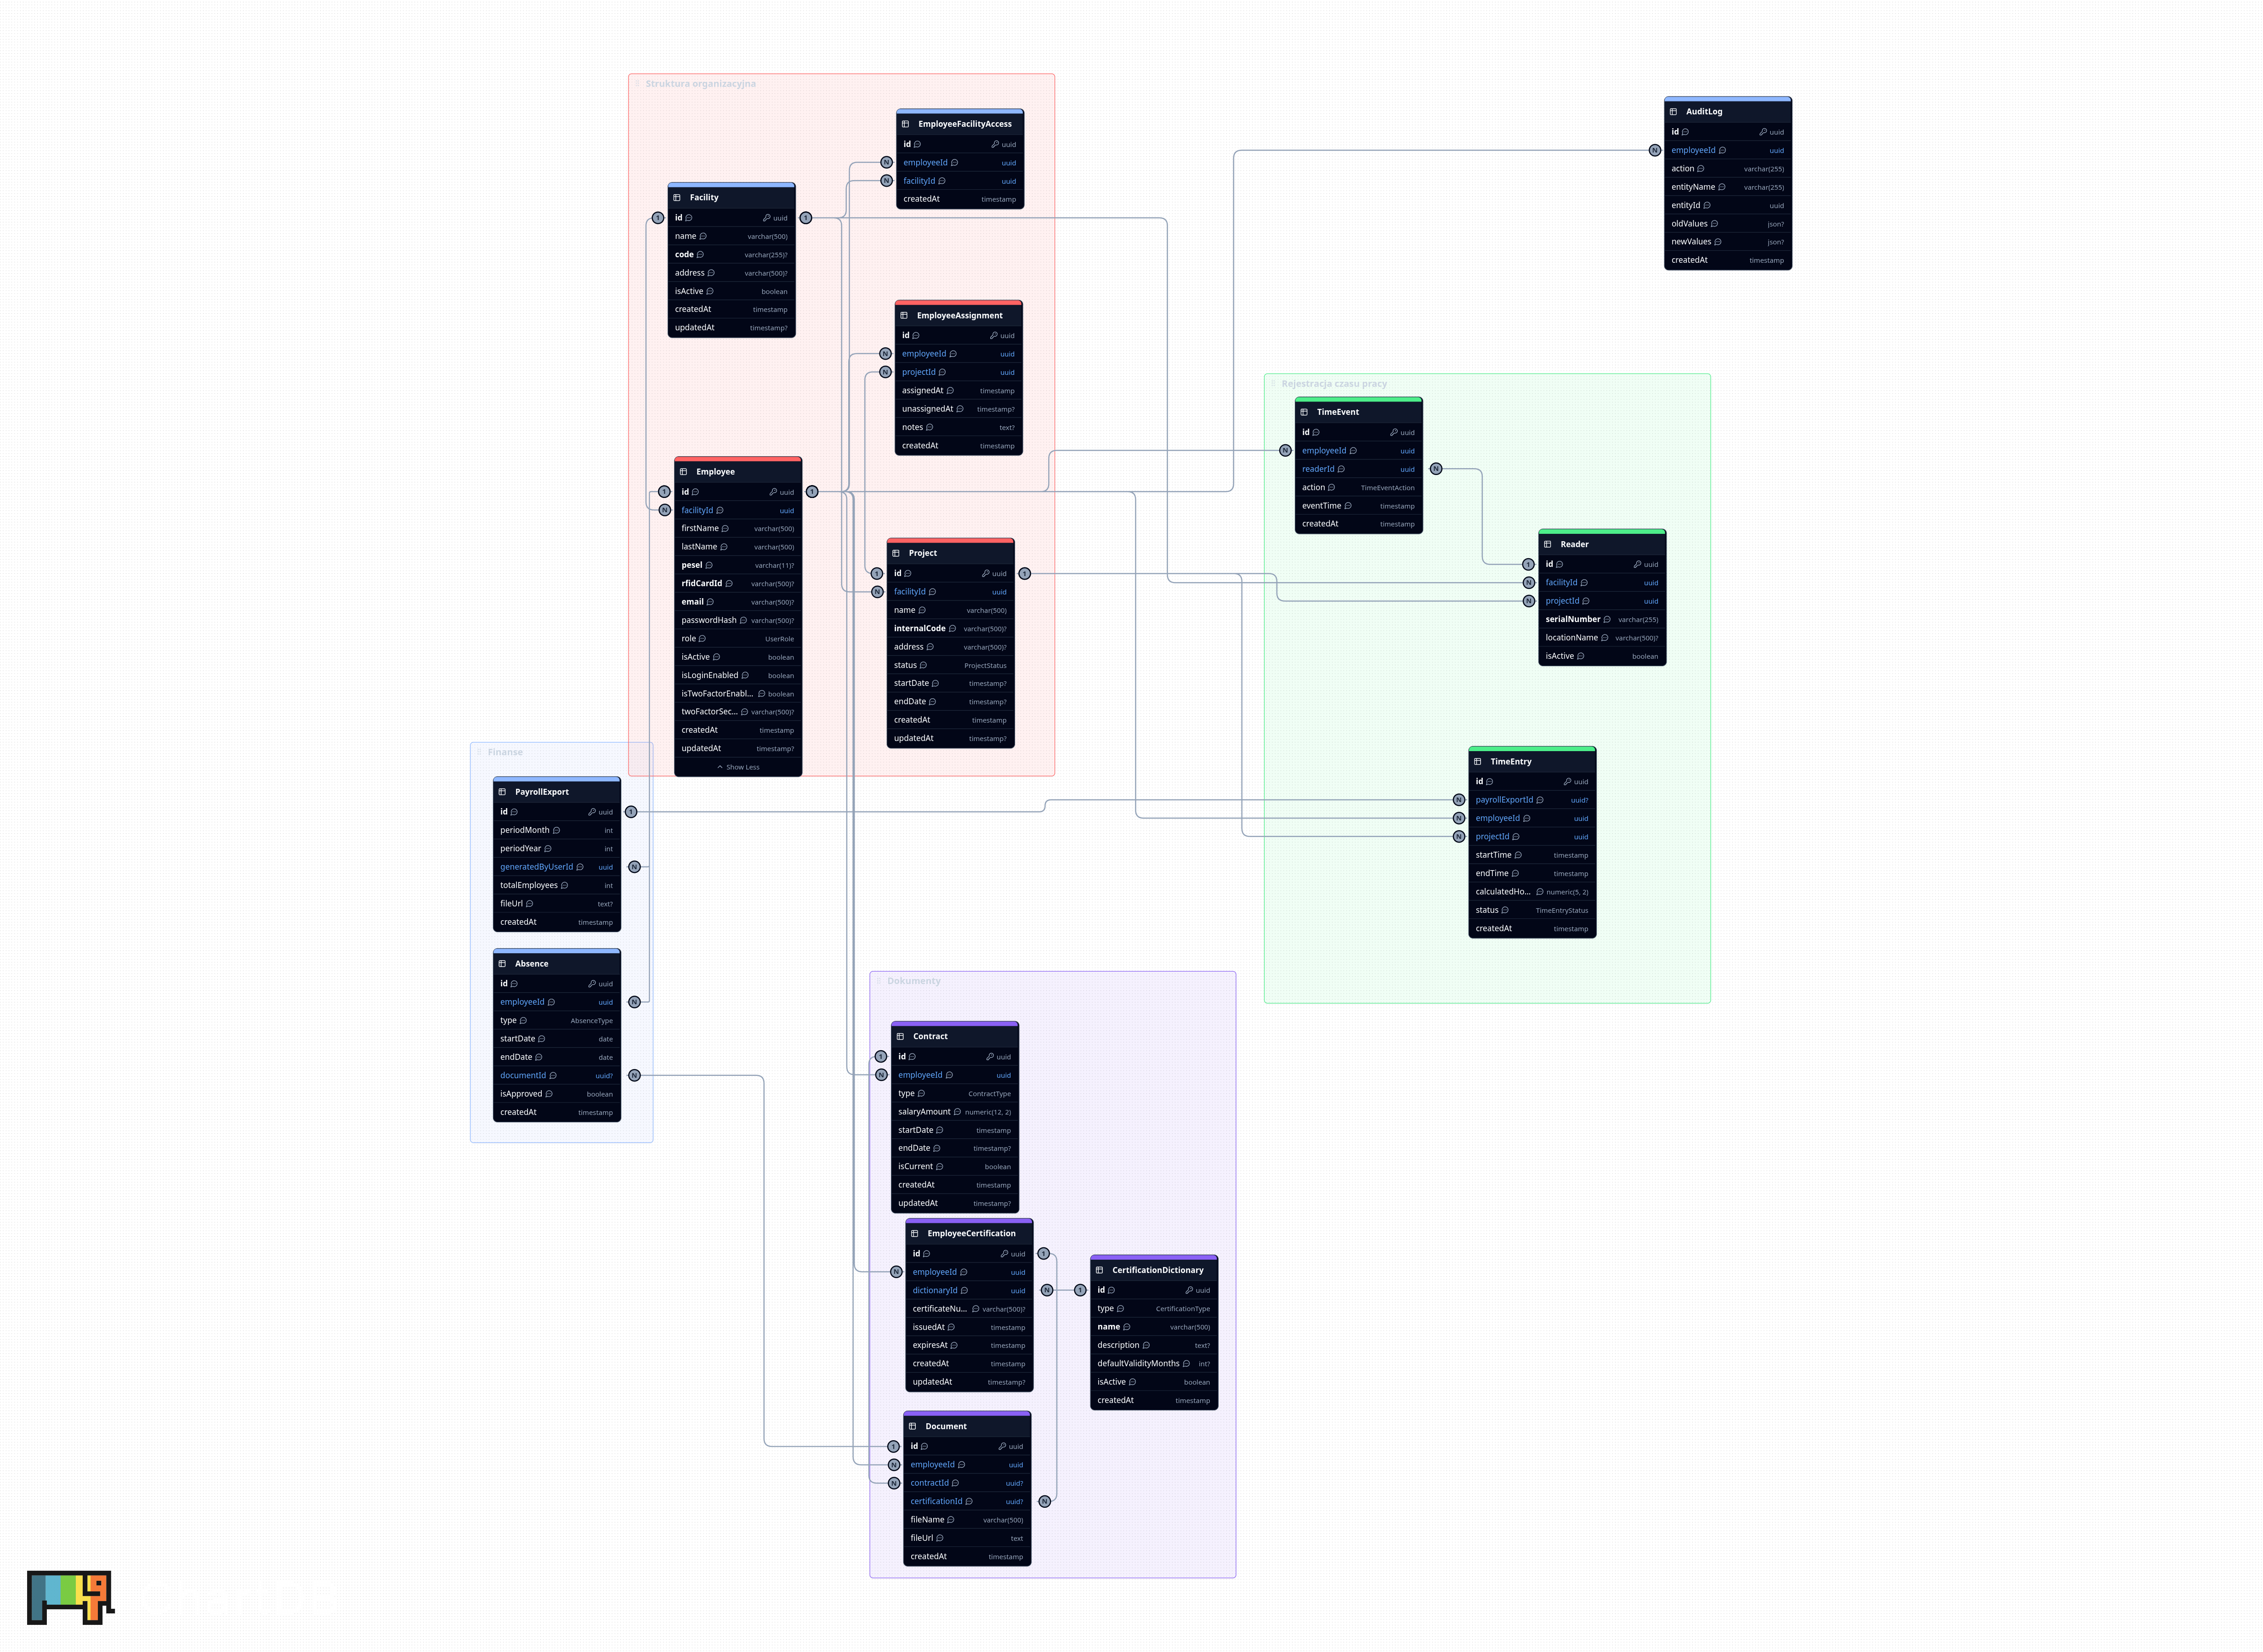
\includegraphics[width=\textwidth, height=0.8\textheight, keepaspectratio]{rys/erd.png} 
    \caption{Logiczny model danych systemu \texttt{WorkFlow}}
    \label{fig:erd_diagram}
\end{figure}

\subsection{Założenia modelu danych}

Podczas projektowania modelu danych przyjęto kilka podstawowych założeń. Pierwszym z nich było zastosowanie identyfikatorów typu \texttt{UUID} jako kluczy głównych. Rozwiązanie to pozwala na jednoznaczne identyfikowanie rekordów i jest wygodne w systemach, które mogą być rozwijane o dodatkowe integracje lub wiele środowisk uruchomieniowych.

Drugim założeniem było rozdzielenie danych źródłowych od danych przetworzonych. Najlepiej widać to w module czasu pracy. Tabela \texttt{TimeEvent} przechowuje surowe zdarzenia pochodzące z czytników RCP, natomiast tabela \texttt{TimeEntry} przechowuje przetworzone wpisy czasu pracy, które mogą być dalej weryfikowane i wykorzystywane w rozliczeniach.

Trzecim założeniem było powiązanie danych z zakładami. Pracownicy, projekty i czytniki RCP są przypisane do zakładu, co pozwala ograniczać zakres widocznych danych w zależności od uprawnień użytkownika.

Model danych został ograniczony do modułów obecnych w aktualnym zakresie projektu. Z tego względu w dokumentacji i diagramie nie uwzględniono modułu sprzętu, ponieważ został on wyłączony z zakresu realizowanej aplikacji.

\subsection{Podział modelu na obszary}

Model danych można podzielić na pięć głównych obszarów logicznych:
\begin{itemize}
    \item \textbf{Struktura organizacyjna} -- obejmuje zakłady, pracowników, dostęp do zakładów, projekty oraz przypisania pracowników do projektów.
    \item \textbf{Rejestracja czasu pracy} -- obejmuje czytniki RCP, surowe zdarzenia wejścia i wyjścia oraz przetworzone wpisy czasu pracy.
    \item \textbf{Kadry i dokumentacja} -- obejmuje umowy, dokumenty, certyfikaty, słownik certyfikatów oraz nieobecności.
    \item \textbf{Rozliczenia} -- obejmuje eksporty payroll oraz powiązanie zatwierdzonych wpisów czasu pracy z paczką rozliczeniową.
    \item \textbf{Audyt} -- obejmuje rejestrowanie wybranych operacji wykonywanych na danych systemu.
\end{itemize}

Taki podział ułatwia analizę modelu oraz pokazuje, które tabele pełnią funkcję centralną, a które są tabelami pomocniczymi lub relacyjnymi.

\subsection{Słownik głównych encji}

W tabeli \ref{tab:main_entities} przedstawiono najważniejsze encje występujące w modelu danych systemu \texttt{WorkFlow}.

\begin{table}[H]
\centering
\renewcommand{\arraystretch}{1.25}
\begin{tabular}{|p{0.24\textwidth}|p{0.68\textwidth}|}
\hline
\textbf{Encja} & \textbf{Znaczenie w systemie} \\ \hline
\texttt{Facility} & Zakład lub jednostka organizacyjna. Do zakładu przypisywani są pracownicy, projekty oraz czytniki RCP. \\ \hline
\texttt{Employee} & Centralna tabela osób. Przechowuje dane pracownika oraz dane konta użytkownika, takie jak e-mail, rola, status aktywności i identyfikator karty RFID. \\ \hline
\texttt{EmployeeFacilityAccess} & Tabela określająca, do których zakładów użytkownik posiada dostęp. Umożliwia obsługę wielu zakładów przez jednego użytkownika. \\ \hline
\texttt{Project} & Projekt, budowa lub miejsce pracy. Jest przypisany do zakładu i może posiadać przypisanych pracowników oraz czytniki RCP. \\ \hline
\texttt{EmployeeAssignment} & Historia przypisań pracowników do projektów. Pozwala określić, kto, od kiedy i do jakiego projektu został przypisany. \\ \hline
\texttt{Reader} & Czytnik RCP. Jest powiązany z zakładem oraz projektem i służy do rejestrowania zdarzeń czasu pracy. \\ \hline
\texttt{TimeEvent} & Surowe zdarzenie z czytnika RCP. Przechowuje informację o pracowniku, czytniku, typie zdarzenia oraz czasie odbicia. \\ \hline
\texttt{TimeEntry} & Przetworzony wpis czasu pracy utworzony na podstawie zdarzeń \texttt{IN} i \texttt{OUT}. Zawiera czas rozpoczęcia, zakończenia, liczbę godzin i status. \\ \hline
\texttt{Contract} & Umowa pracownika. Przechowuje typ umowy, wynagrodzenie, daty obowiązywania oraz informację, czy umowa jest aktualna. \\ \hline
\texttt{CertificationDictionary} & Słownik typów certyfikatów, szkoleń, badań i uprawnień. \\ \hline
\texttt{EmployeeCertification} & Konkretny certyfikat przypisany do pracownika, wraz z datą wydania i datą ważności. \\ \hline
\texttt{Absence} & Nieobecność pracownika, na przykład urlop, L4, nieobecność nieusprawiedliwiona lub specjalna. \\ \hline
\texttt{Document} & Metadane dokumentu pracownika. Plik przechowywany jest w MinIO, a baza przechowuje jego nazwę, lokalizację i powiązania. \\ \hline
\texttt{PayrollExport} & Eksport rozliczeniowy obejmujący zatwierdzone wpisy czasu pracy dla danego okresu. \\ \hline
\texttt{AuditLog} & Rejestr wybranych operacji wykonanych w systemie. Przechowuje akcję, encję, identyfikator rekordu oraz wartości przed i po zmianie. \\ \hline
\end{tabular}
\caption{Główne encje modelu danych systemu \texttt{WorkFlow}}
\label{tab:main_entities}
\end{table}

\subsection{Struktura organizacyjna}

Podstawą modelu organizacyjnego jest tabela \texttt{Facility}. Reprezentuje ona zakład lub jednostkę organizacyjną. Z zakładem powiązani są pracownicy, projekty oraz czytniki RCP. Dzięki temu dane można grupować według lokalizacji lub oddziałów.

Tabela \texttt{Employee} pełni podwójną rolę. Z jednej strony przechowuje dane pracownika, takie jak imię, nazwisko, PESEL, status aktywności i identyfikator karty RFID. Z drugiej strony zawiera pola potrzebne do logowania, takie jak adres e-mail, hash hasła, rola systemowa oraz flaga określająca, czy logowanie jest włączone.

Dostęp użytkowników do zakładów został opisany w tabeli \texttt{EmployeeFacilityAccess}. Dzięki temu użytkownik może posiadać dostęp do więcej niż jednego zakładu. Jest to istotne szczególnie dla administratora, HR lub księgowości, którzy mogą obsługiwać dane wielu jednostek.

Relacja pomiędzy pracownikiem a projektem została zrealizowana przez tabelę \texttt{EmployeeAssignment}. Tabela ta umożliwia przechowywanie historii przypisań, a nie tylko aktualnego stanu. Dzięki temu można określić, w jakim okresie pracownik był związany z danym projektem.

\subsection{Rejestracja czasu pracy}

Moduł czasu pracy składa się z trzech głównych tabel: \texttt{Reader}, \texttt{TimeEvent} oraz \texttt{TimeEntry}.

Tabela \texttt{Reader} przechowuje informacje o czytniku RCP. Czytnik posiada numer seryjny, nazwę lokalizacji oraz powiązanie z zakładem i projektem. Oznacza to, że zdarzenie odbicia karty na czytniku można powiązać nie tylko z pracownikiem, ale również z miejscem pracy.

Tabela \texttt{TimeEvent} przechowuje surowe zdarzenia z czytników. Każde zdarzenie zawiera pracownika, czytnik, typ zdarzenia oraz czas zdarzenia. Typ zdarzenia jest ograniczony do dwóch wartości: \texttt{IN} oraz \texttt{OUT}.

Tabela \texttt{TimeEntry} przechowuje dane przetworzone. Wpis czasu pracy powstaje na podstawie pary zdarzeń wejścia i wyjścia. Zawiera on czas rozpoczęcia, czas zakończenia, wyliczoną liczbę godzin, projekt oraz status wpisu.

\begin{table}[H]
\centering
\renewcommand{\arraystretch}{1.25}
\begin{tabular}{|p{0.24\textwidth}|p{0.20\textwidth}|p{0.44\textwidth}|}
\hline
\textbf{Pole} & \textbf{Typ} & \textbf{Opis} \\ \hline
\texttt{id} & UUID & Klucz główny wpisu czasu pracy. \\ \hline
\texttt{payrollExportId} & UUID, opcjonalny & Powiązanie z eksportem rozliczeniowym, jeżeli wpis został już ujęty w paczce payroll. \\ \hline
\texttt{employeeId} & UUID & Pracownik, którego dotyczy wpis czasu pracy. \\ \hline
\texttt{projectId} & UUID & Projekt, na którym pracownik wykonywał pracę. \\ \hline
\texttt{startTime} & timestamp & Czas rozpoczęcia pracy. \\ \hline
\texttt{endTime} & timestamp & Czas zakończenia pracy. \\ \hline
\texttt{calculatedHours} & numeric(5,2) & Wyliczona liczba przepracowanych godzin. \\ \hline
\texttt{status} & \texttt{TimeEntryStatus} & Status wpisu czasu pracy: \texttt{PENDING}, \texttt{APPROVED} lub \texttt{REJECTED}. \\ \hline
\texttt{createdAt} & timestamp & Data utworzenia wpisu. \\ \hline
\end{tabular}
\caption{Struktura tabeli \texttt{TimeEntry}}
\label{tab:timeentry_struct}
\end{table}

Rozdzielenie \texttt{TimeEvent} i \texttt{TimeEntry} jest ważne projektowo. Pozwala zachować pierwotne dane z urządzenia, a jednocześnie tworzyć dane robocze, które mogą być zatwierdzane, odrzucane lub eksportowane do rozliczeń.

\subsection{Kadry i dokumentacja}

Dane kadrowe zostały rozbite na kilka tabel, aby uniknąć przechowywania wszystkich informacji bezpośrednio w tabeli pracownika. Takie podejście poprawia czytelność modelu i umożliwia przechowywanie historii.

Tabela \texttt{Contract} przechowuje umowy pracownika. Każda umowa posiada typ, kwotę wynagrodzenia, datę rozpoczęcia, opcjonalną datę zakończenia oraz informację, czy jest aktualna. Pozwala to przechowywać zarówno bieżące, jak i historyczne warunki zatrudnienia.

Tabele \texttt{CertificationDictionary} i \texttt{EmployeeCertification} obsługują certyfikaty, badania i szkolenia. Pierwsza tabela definiuje słownik możliwych certyfikatów, natomiast druga przechowuje konkretne certyfikaty przypisane do pracowników. Dzięki temu można kontrolować daty ważności dokumentów.

Tabela \texttt{Absence} przechowuje nieobecności pracowników. Zawiera typ nieobecności, zakres dat, status zatwierdzenia oraz opcjonalne powiązanie z dokumentem.

Tabela \texttt{Document} przechowuje metadane dokumentów. Sam plik nie jest zapisywany bezpośrednio w bazie danych. W bazie przechowywana jest nazwa pliku, adres lub ścieżka do pliku oraz powiązanie z pracownikiem, umową lub certyfikatem.

\subsection{Rozliczenia}

Tabela \texttt{PayrollExport} reprezentuje paczkę danych rozliczeniowych dla danego miesiąca i roku. Przechowuje informację o użytkowniku, który wygenerował eksport, liczbie pracowników objętych eksportem oraz opcjonalnej ścieżce do pliku eksportu.

Z tabelą \texttt{PayrollExport} powiązana jest tabela \texttt{TimeEntry}. Jeżeli pole \texttt{payrollExportId} w tabeli \texttt{TimeEntry} jest wypełnione, oznacza to, że dany wpis czasu pracy został ujęty w konkretnej paczce rozliczeniowej. Takie rozwiązanie ogranicza ryzyko ponownego rozliczenia tych samych godzin.

\subsection{Audit log}

Tabela \texttt{AuditLog} została przewidziana do rejestrowania wybranych operacji wykonywanych na danych systemu. Każdy wpis audytowy zawiera użytkownika wykonującego operację, nazwę akcji, nazwę encji, identyfikator rekordu oraz opcjonalnie wartości przed zmianą i po zmianie.

Zastosowanie pól typu \texttt{Json} pozwala przechowywać zmiany w elastycznej formie, bez konieczności tworzenia osobnych tabel dla każdego rodzaju operacji. Mechanizm ten jest szczególnie przydatny przy analizie zmian dotyczących danych kadrowych, umów lub wpisów czasu pracy.

\subsection{Typy wyliczeniowe}

W modelu danych zastosowano kilka typów wyliczeniowych, które ograniczają możliwe wartości wybranych pól. Dzięki temu baza danych nie przyjmuje przypadkowych wartości tekstowych, a aplikacja może opierać się na stałym zbiorze statusów i kategorii.

Najważniejsze typy wyliczeniowe to:
\begin{itemize}
    \item \texttt{UserRole} -- role użytkowników: \texttt{ADMIN}, \texttt{HR}, \texttt{OFFICE}, \texttt{FOREMAN}, \texttt{ACCOUNTING}, \texttt{WORKER},
    \item \texttt{ProjectStatus} -- statusy projektów: \texttt{PLANNED}, \texttt{ACTIVE}, \texttt{COMPLETED}, \texttt{SUSPENDED},
    \item \texttt{TimeEventAction} -- typy zdarzeń RCP: \texttt{IN}, \texttt{OUT},
    \item \texttt{TimeEntryStatus} -- statusy wpisów czasu pracy: \texttt{PENDING}, \texttt{APPROVED}, \texttt{REJECTED},
    \item \texttt{ContractType} -- typy umów: \texttt{UOP}, \texttt{UZ}, \texttt{UD}, \texttt{B2B},
    \item \texttt{CertificationType} -- typy certyfikatów: \texttt{BHP}, \texttt{MEDICAL}, \texttt{UDT}, \texttt{OTHER},
    \item \texttt{AbsenceType} -- typy nieobecności: \texttt{HOLIDAY}, \texttt{SICK\_LEAVE}, \texttt{UNEXCUSED}, \texttt{SPECIAL}.
\end{itemize}

\subsection{Implementacja fizyczna bazy danych}

Fizyczna struktura bazy danych jest generowana na podstawie modeli Prisma. Przykładowa definicja tabeli \texttt{TimeEntry} w schemacie Prisma wygląda następująco:

\begin{lstlisting}[language=SQL, caption=Fragment modelu TimeEntry w schemacie Prisma]
model TimeEntry {
  id              String          @id @default(dbgenerated("gen_random_uuid()")) @db.Uuid
  payrollExportId String?         @db.Uuid
  employeeId      String          @db.Uuid
  projectId       String          @db.Uuid
  startTime       DateTime        @db.Timestamp(6)
  endTime         DateTime        @db.Timestamp(6)
  calculatedHours Decimal         @db.Decimal(5, 2)
  status          TimeEntryStatus @default(PENDING)
  createdAt       DateTime        @default(now()) @db.Timestamp(6)

  payrollExport   PayrollExport?  @relation(fields: [payrollExportId], references: [id])
  employee        Employee        @relation(fields: [employeeId], references: [id])
  project         Project         @relation(fields: [projectId], references: [id])
}
\end{lstlisting}

W praktyce struktura bazy może zostać zsynchronizowana z modelem Prisma za pomocą polecenia:

\begin{lstlisting}[language=bash, caption=Synchronizacja bazy danych ze schematem Prisma]
docker compose -f docker-compose.prod.yml --env-file .env exec backend npx prisma db push --config prisma.config.ts
\end{lstlisting}

Takie podejście pozwala utrzymać jedno źródło prawdy dla struktury bazy danych w kodzie projektu.

\subsection{Strategia dostępu do danych}

Backend komunikuje się z bazą danych za pomocą Prisma ORM. Prisma odpowiada za mapowanie modeli aplikacji na tabele bazy danych, wykonywanie zapytań oraz obsługę relacji pomiędzy encjami.

W projekcie większość operacji może być realizowana przez standardowe zapytania ORM. Dotyczy to między innymi dodawania pracowników, edycji danych, pobierania list, tworzenia umów, certyfikatów, nieobecności oraz wpisów czasu pracy.

W przypadku bardziej złożonych raportów lub eksportów możliwe jest wykorzystanie zapytań agregujących. Aktualna wersja projektu skupia się jednak przede wszystkim na czytelnym modelu relacyjnym i poprawnym powiązaniu danych, a nie na zaawansowanej analityce SQL.

\subsection{Znaczenie modelu danych dla systemu}

Model danych systemu \texttt{WorkFlow} został zaprojektowany tak, aby odwzorować podstawowe zależności występujące w procesach kadrowych i ewidencji czasu pracy. Najważniejszą encją jest pracownik, który łączy się z większością pozostałych obszarów systemu: zakładami, projektami, dokumentami, certyfikatami, umowami, nieobecnościami i czasem pracy.

Dzięki relacyjnemu modelowi danych system może zachować spójność pomiędzy modułami. Przykładowo wpis czasu pracy nie istnieje samodzielnie, lecz jest powiązany z pracownikiem i projektem. Dokument nie jest anonimowym plikiem, lecz posiada właściciela i może być powiązany z umową lub certyfikatem. Certyfikat nie jest tylko tekstową informacją, ale wynika ze słownika i posiada datę ważności.

Takie ustrukturyzowanie danych umożliwia dalszy rozwój systemu, między innymi o dodatkowe raporty, powiadomienia, integracje księgowe lub bardziej rozbudowane mechanizmy kontroli dostępu.